\documentclass[aspectratio=169]{beamer}
%\usetheme{CambridgeUS}
%\usecolortheme{beaver}

%\usefonttheme{serif}
%\usepackage{helvet}

\usefonttheme{serif}     % Font theme: serif
%\usepackage{ccfonts}     % Font family: Concrete Math
\usepackage[T1]{fontenc} % Font encoding: T1

\setbeamersize{text margin left=42pt,text margin right=42pt} 
\setbeamertemplate{navigation symbols}{}
\setbeamertemplate{itemize items}[default]

\beamertemplatenavigationsymbolsempty

\definecolor{fore}{RGB}{51,51,51}
\definecolor{back}{RGB}{255, 254, 250}
\definecolor{title}{RGB}{ 255, 15, 0}
\definecolor{links}{RGB}{18, 168, 255}

\setbeamercolor{titlelike}{fg=title}
\setbeamercolor{normal text}{fg=fore,bg=back}
\setbeamercolor{alerted text}{fg=title}
\setbeamercolor{itemize item}{fg=title}
\setbeamercolor{enumerate item}{fg=title}
\hypersetup{colorlinks,urlcolor=links}

% for code https://kbroman.org/blog/2013/10/07/better-looking-latexbeamer-slides/
\usepackage{listings}
\definecolor{keywords}{RGB}{255,0,90}
\definecolor{comments}{RGB}{60,179,113}
\lstset{language=Python,
keywordstyle=color{keywords},
commentstyle=color{comments}emph}

% fonts
\usepackage[sc]{mathpazo}


% title info
\title{\textbf{Cycling \& Walking:}}
\subtitle{\textbf{GGR424 - Transportation Geography \& Planning}}
\author{Jeff Allen}
\institute{University of Toronto}
\date{January 24, 2022}


\begin{document}
	
\begin{frame}
	\titlepage	
\end{frame}




\begin{frame}
	\begin{columns}
		\begin{column}{0.5\textwidth}
			
			\textbf{Today:}
			\begin{itemize}
				\item Benefits of active travel
				
				\item Safety issues and other concerns
				
				\item "Micro" design improvements
				
				\item Designing "complete streets"
				
				\item Networks \& connectivity
			\end{itemize}
			
		\end{column}
		
		\begin{column}{0.5\textwidth}
			\begin{figure}
				\centering
				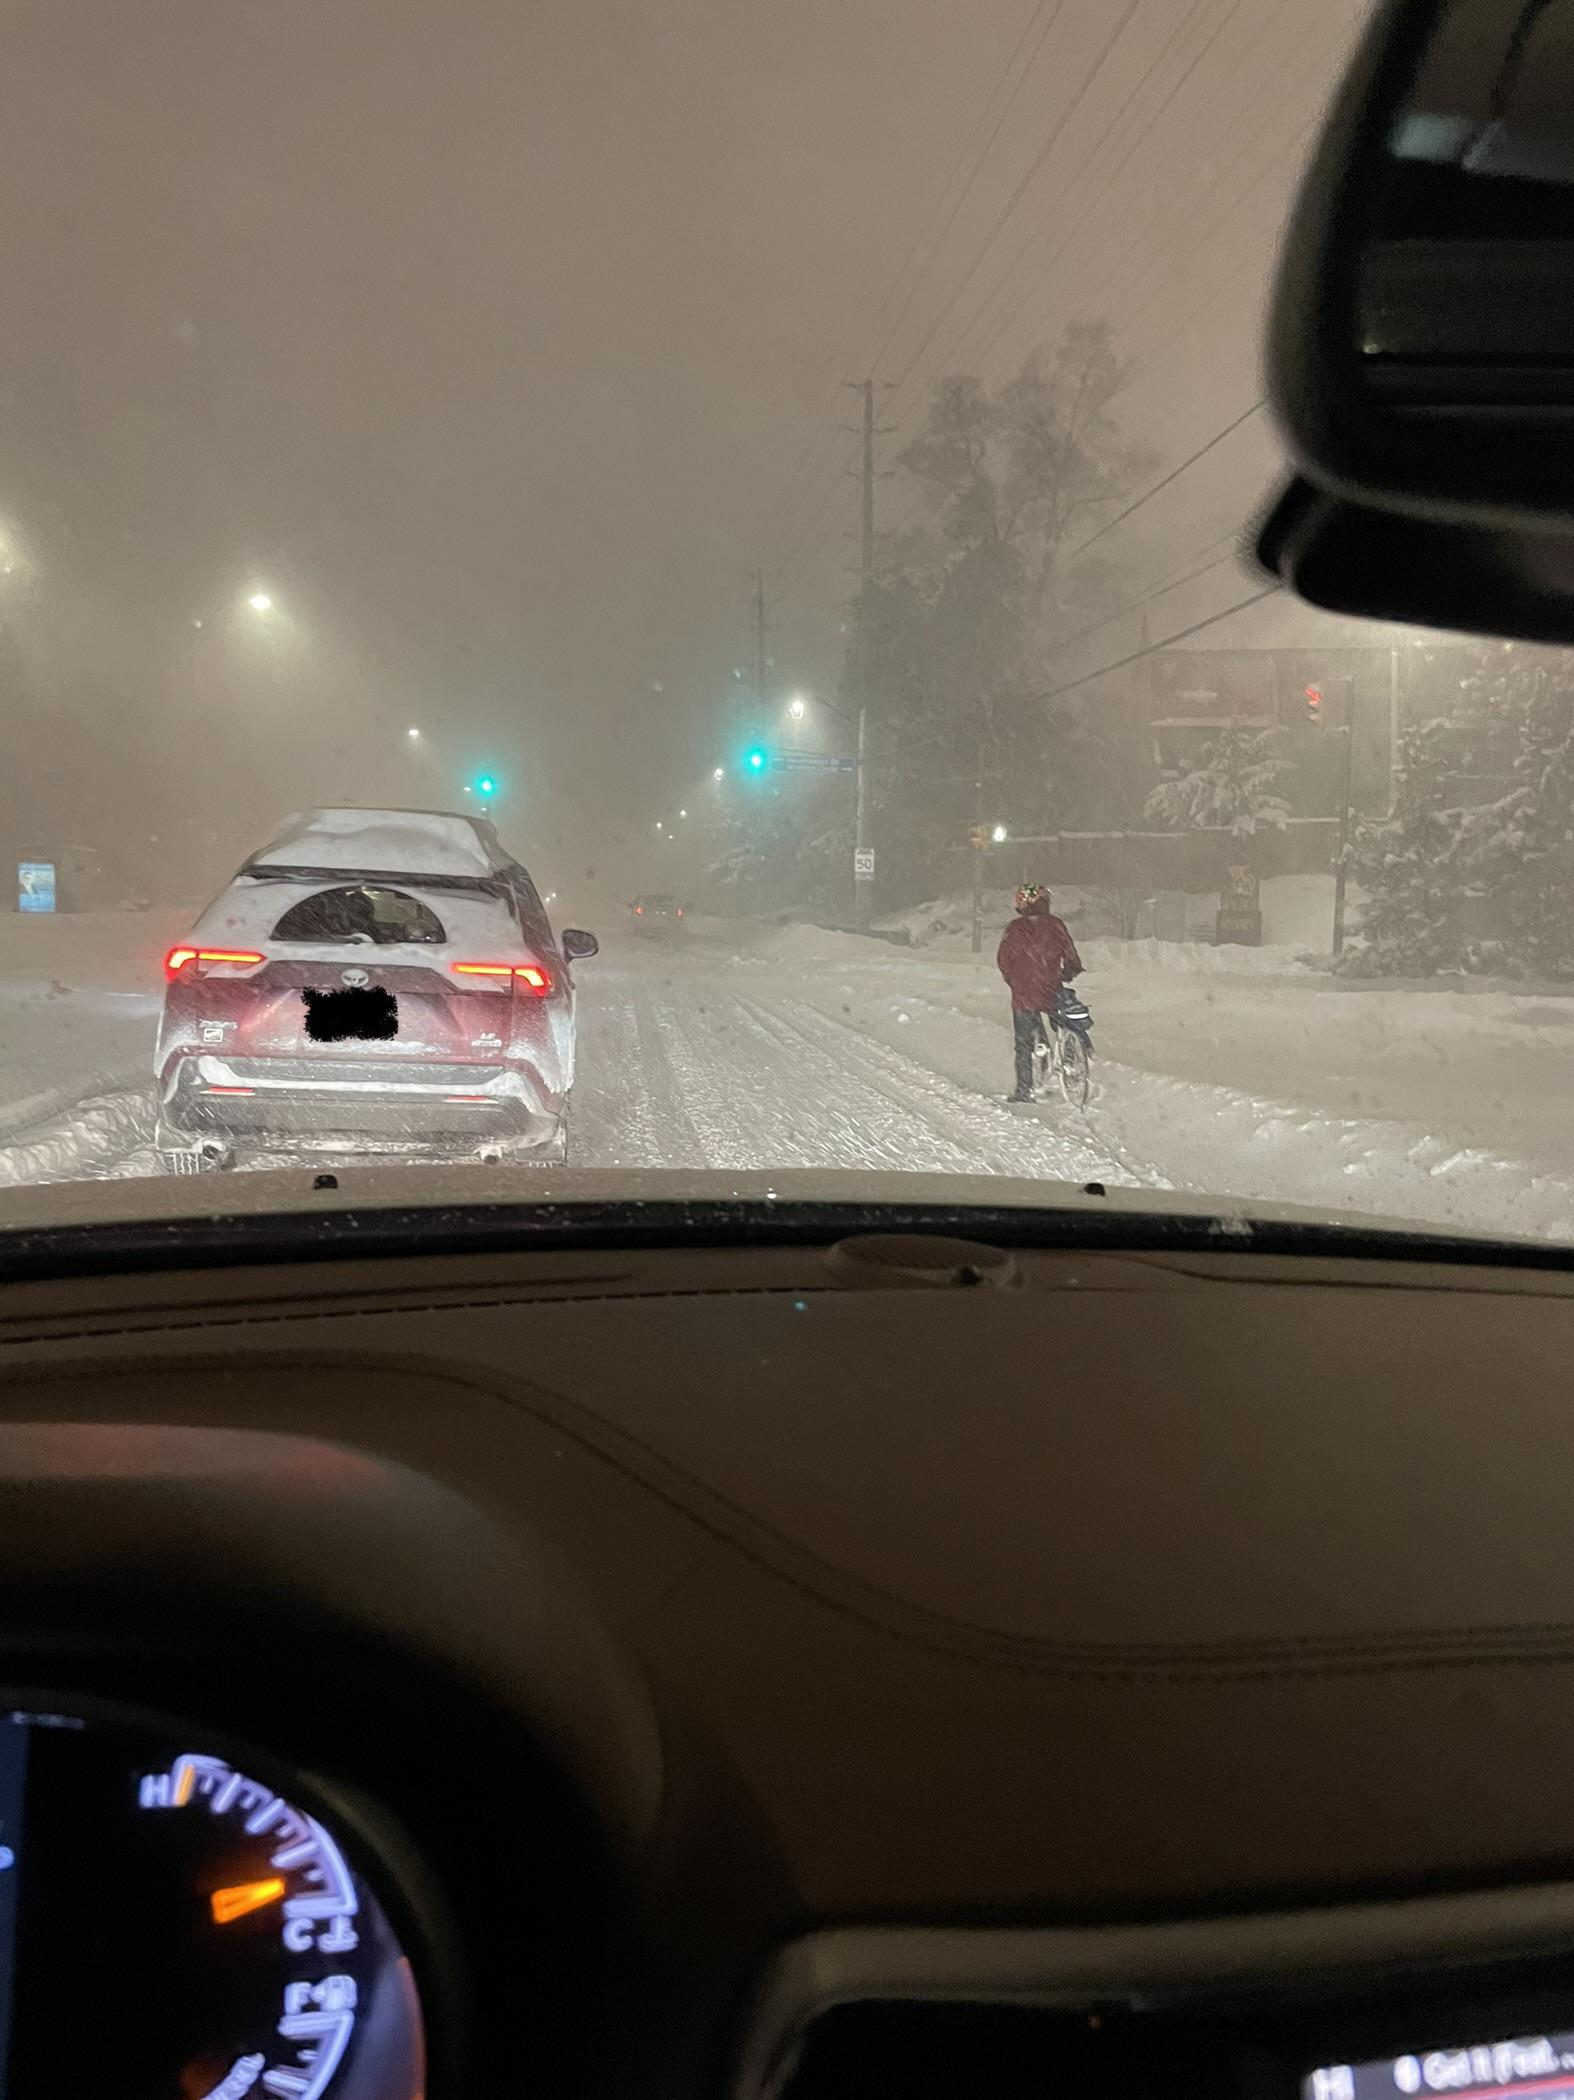
\includegraphics[width=1\linewidth]{images/bike_winter.jpg}
			\end{figure}
			
		\end{column}
		
		
		
	\end{columns}
\end{frame}




\begin{frame}
	
	\textbf{Active travel} - non-motorized mobility
	
	\vspace{4mm}
	
	e.g. walking and cycling, but also rollerblading, skateboarding, ice-skating, kick scooters, cross-country skiing, etc.
	
	\vspace{4mm}
	
	Can be ...
	\begin{itemize}
		\item for recreation
		\item for travelling to a location
	\end{itemize}
		
\end{frame}




\begin{frame}
	
	\textbf{Benefits of Active Travel}
	
	\vspace{4mm}
	
	Can replace trips by other modes (driving, transit), meaning reduced congestion, pollution, GHG emissions, etc.
	
	\begin{figure}
		\centering
		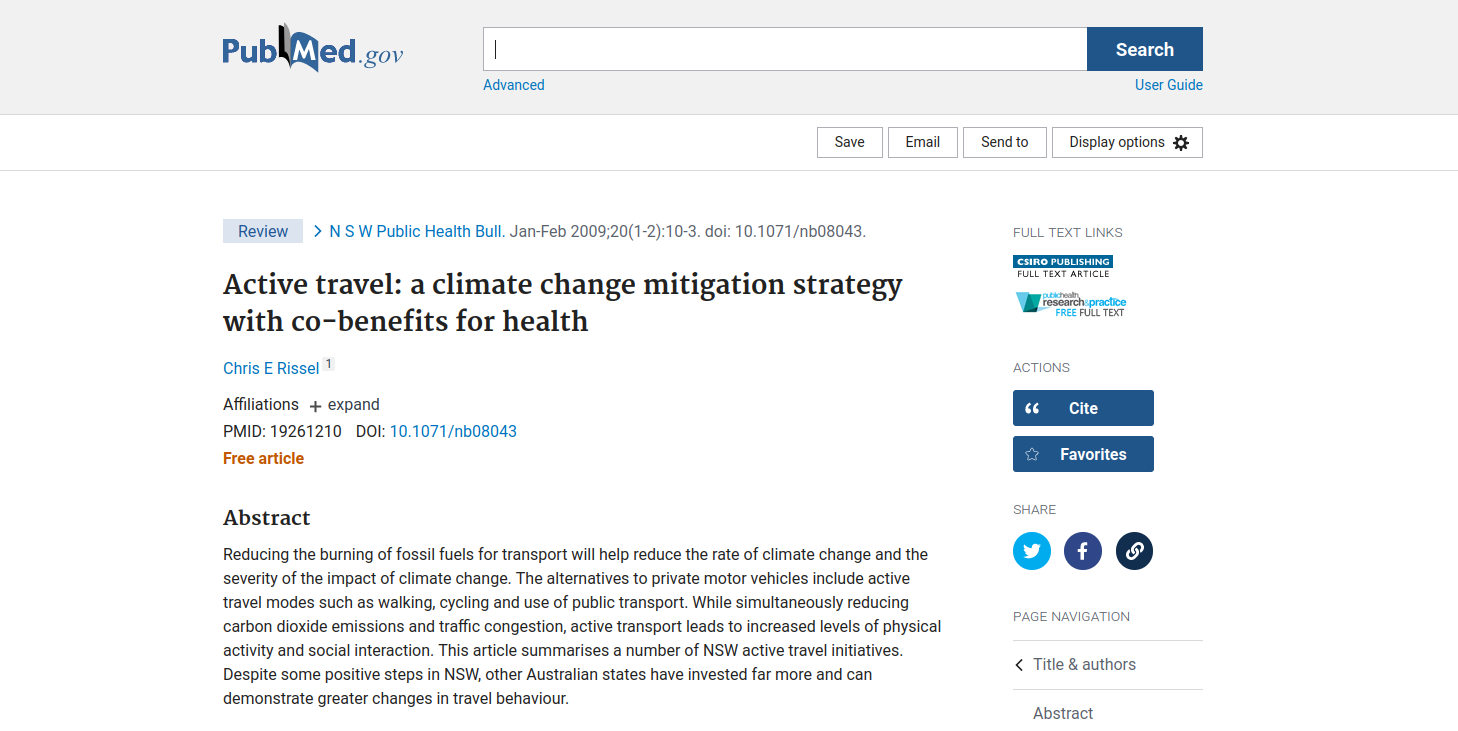
\includegraphics[width=0.7\linewidth]{images/active_travel_pollution.png}
	\end{figure}
	
	\tiny\url{https://pubmed.ncbi.nlm.nih.gov/19261210/}

\end{frame}



\begin{frame}
	
	\textbf{Benefits of Active Travel}
	
	\vspace{4mm}
	
	Plenty of research highlights health benefits of active travel, e.g. 
	
	\begin{figure}
		\centering
		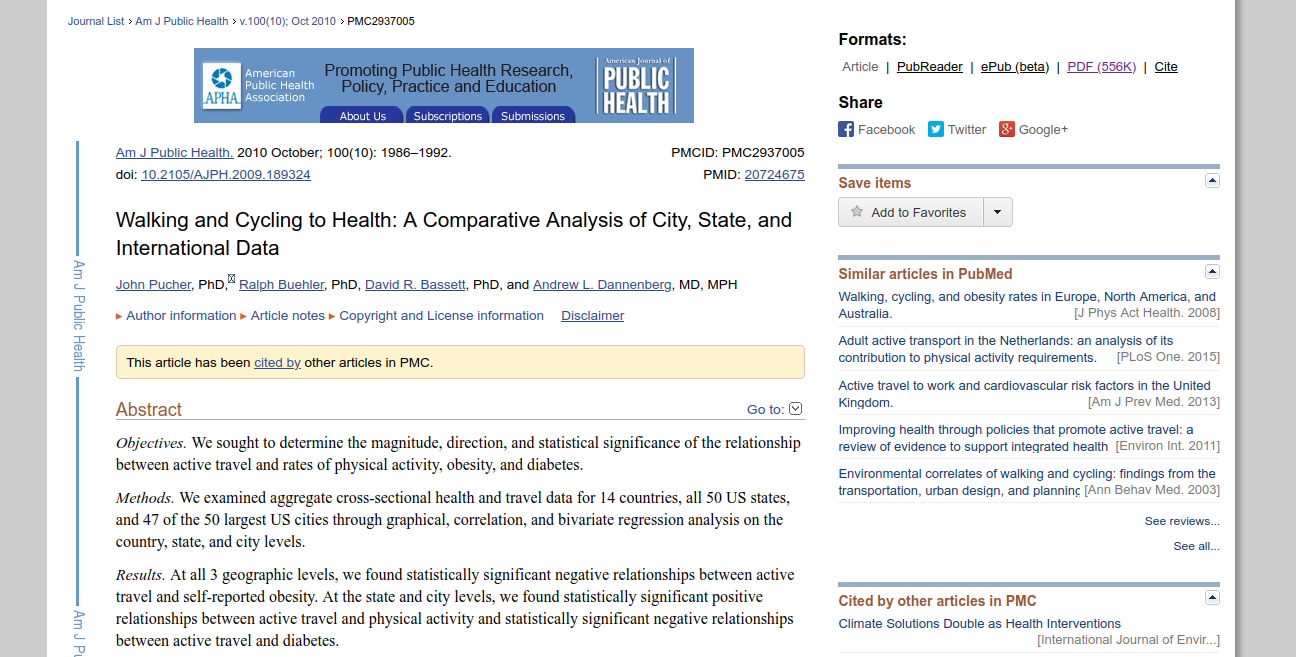
\includegraphics[width=1\linewidth]{images/health_ben_active_travel.png}
	\end{figure}
	
\end{frame}




\begin{frame}
	
	\textbf{Benefits of Active Travel}
	
	\vspace{4mm}
	
	Increased "enjoyment" or "satisfaction" of travel
	
	\begin{figure}
		\centering
		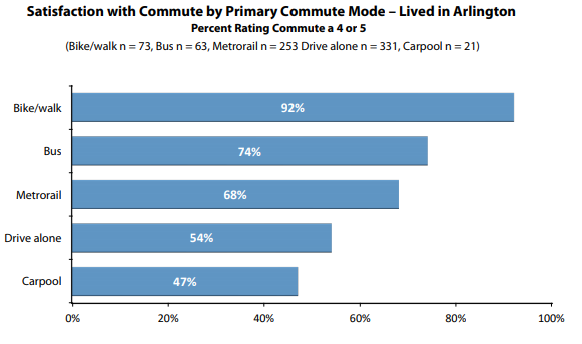
\includegraphics[width=0.7\linewidth]{images/mode_satisfaction.png}
	\end{figure}

	\tiny\url{https://mobilitylab.org/2020/09/29/the-pursuit-of-happiness-how-commute-mode-affects-commute-mood/}
	
\end{frame}



\begin{frame}
	
	\textbf{Benefits of Active Travel}
	
	\vspace{4mm}
	
	\small{"studies indicate that creating or improving active travel facilities generally has positive or non-significant economic impacts on retail"}
	
	\begin{figure}
		\centering
		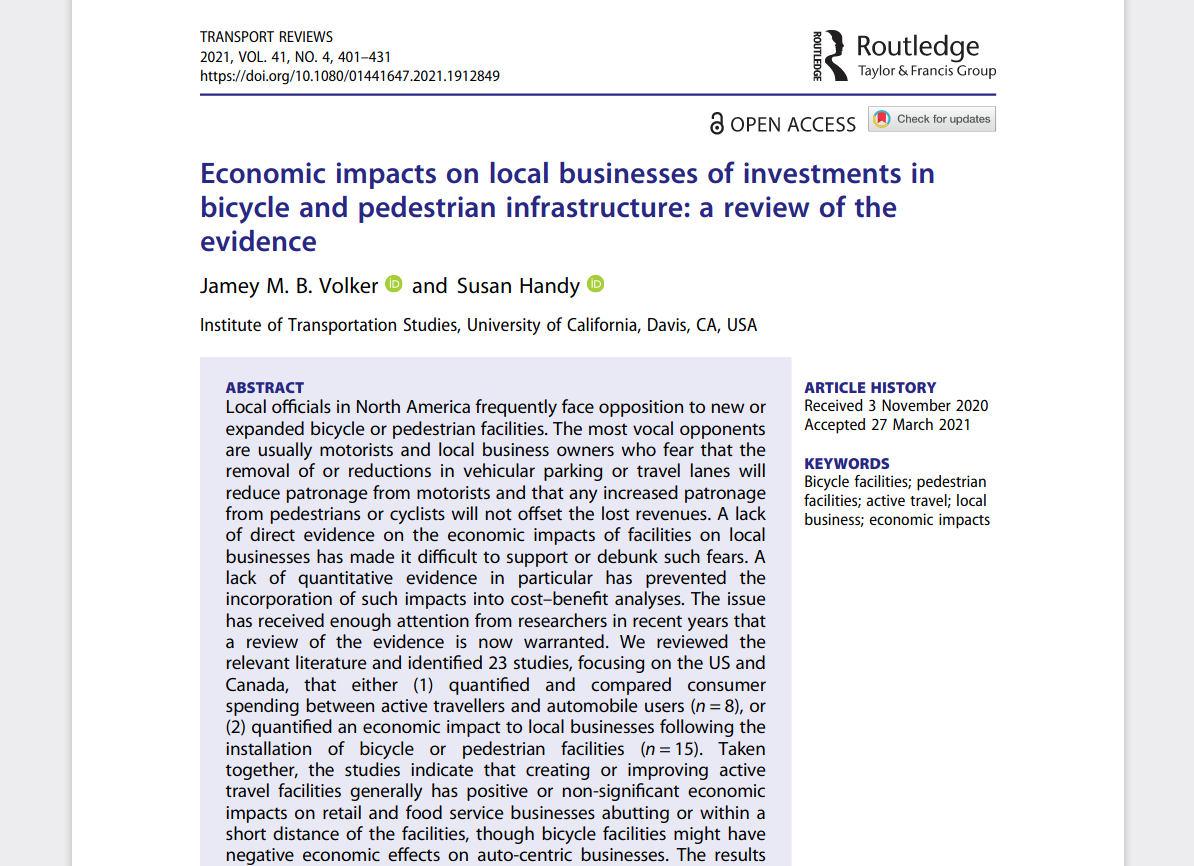
\includegraphics[width=0.6\linewidth]{images/economic_impacts_active_travel.png}
	\end{figure}
	
	\tiny\url{https://doi.org/10.1080/01441647.2021.1912849}
	
\end{frame}




%\begin{frame}
%	
%	\textbf{What are some other benefits of active travel?}
%
%\end{frame}





\begin{frame}
	
	\textbf{What deters active travel?}
	
\end{frame}






\begin{frame}
	
	\textbf{Induced demand, not just for cars!}
	
	
	
\end{frame}







\begin{frame}
	\textbf{Next Week} 
	
	\vspace{4mm}
	
	Public Transit
	
	\begin{itemize}
				
		
		\item etc.
				
		
	\end{itemize}
	
\end{frame}




\end{document}